\documentclass[ucs,9pt]{beamer}

% Copyright 2004 by Till Tantau <tantau@users.sourceforge.net>.
%
% In principle, this file can be redistributed and/or modified under
% the terms of the GNU Public License, version 2.
%
% However, this file is supposed to be a template to be modified
% for your own needs. For this reason, if you use this file as a
% template and not specifically distribute it as part of a another
% package/program, I grant the extra permission to freely copy and
% modify this file as you see fit and even to delete this copyright
% notice.
%
% Modified by Tobias G. Pfeiffer <tobias.pfeiffer@math.fu-berlin.de>
% to show usage of some features specific to the FU Berlin template.

% remove this line and the "ucs" option to the documentclass when your editor is not utf8-capable
\usepackage[utf8x]{inputenc}    % to make utf-8 input possible
\usepackage[english]{babel}     % hyphenation etc., alternatively use 'german' as parameter

% Template for talks using the Corporate Design of the Freie Universitaet
%   Berlin, created following the guidelines on www.fu-berlin.de/cd by
%   Tobias G. Pfeiffer, <tobias.pfeiffer@math.fu-berlin.de>
% This file can be redistributed and/or modified in any way you like.
%   If you feel you have done significant improvements to this template,
%   please consider providing your modified version to
%   https://www.mi.fu-berlin.de/w/Mi/BeamerTemplateCorporateDesign

\usepackage{amsmath,dsfont,listings}

%%% FU logo
% small version for upper right corner of normal pages
\pgfdeclareimage[height=0.9cm]{university-logo}{FULogo_RGB}
\logo{\pgfuseimage{university-logo}}
% large version for upper right corner of title page
\pgfdeclareimage[height=1.085cm]{big-university-logo}{FULogo_RGB}
\newcommand{\titleimage}[1]{\pgfdeclareimage[height=2.92cm]{title-image}{#1}}
\titlegraphic{\pgfuseimage{title-image}}
%%% end FU logo

% NOTE: 1cm = 0.393 in = 28.346 pt;    1 pt = 1/72 in = 0.0352 cm
\setbeamersize{text margin right=3.5mm, text margin left=7.5mm}  % text margin

% colors to be used
\definecolor{text-grey}{rgb}{0.45, 0.45, 0.45} % grey text on white background
\definecolor{bg-grey}{rgb}{0.66, 0.65, 0.60} % grey background (for white text)
\definecolor{fu-blue}{RGB}{0, 51, 102} % blue text
\definecolor{fu-green}{RGB}{153, 204, 0} % green text
\definecolor{fu-red}{RGB}{204, 0, 0} % red text (used by \alert)

% switch off the sidebars
% TODO: loading \useoutertheme{sidebar} (which is maybe wanted) also inserts
%   a sidebar on title page (unwanted), also indents the page title (unwanted?),
%   and duplicates the navigation symbols (unwanted)
\setbeamersize{sidebar width left=0cm, sidebar width right=0mm}
\setbeamertemplate{sidebar right}{}
\setbeamertemplate{sidebar left}{}
%    XOR
% \useoutertheme{sidebar}

% frame title
% is truncated before logo and splits on two lines
% if neccessary (or manually using \\)
\setbeamertemplate{frametitle}{%
    \vskip-30pt \color{text-grey}\large%
    \begin{minipage}[b][23pt]{80.5mm}%
    \flushleft\insertframetitle%
    \end{minipage}%
}

%%% title page
% TODO: get rid of the navigation symbols on the title page.
%   actually, \frame[plain] *should* remove them...
\setbeamertemplate{title page}{
% upper right: FU logo
\vskip2pt\hfill\pgfuseimage{big-university-logo} \\
\vskip6pt\hskip3pt
% title image of the presentation
\begin{minipage}{11.6cm}
\hspace{-1mm}\inserttitlegraphic
\end{minipage}

% set the title and the author
\vskip14pt
\parbox[top][1.35cm][c]{11cm}{\color{text-grey}\inserttitle \\ \small \insertsubtitle}
\vskip11pt
\parbox[top][1.35cm][c]{11cm}{\small \insertauthor \\ \insertinstitute \\[3mm] \insertdate}
}
%%% end title page

%%% colors
\usecolortheme{lily}
\setbeamercolor*{normal text}{fg=black,bg=white}
\setbeamercolor*{alerted text}{fg=fu-red}
\setbeamercolor*{example text}{fg=fu-green}
\setbeamercolor*{structure}{fg=fu-blue}

\setbeamercolor*{block title}{fg=white,bg=black!50}
\setbeamercolor*{block title alerted}{fg=white,bg=black!50}
\setbeamercolor*{block title example}{fg=white,bg=black!50}

\setbeamercolor*{block body}{bg=black!10}
\setbeamercolor*{block body alerted}{bg=black!10}
\setbeamercolor*{block body example}{bg=black!10}

\setbeamercolor{bibliography entry author}{fg=fu-blue}
% TODO: this doesn't work at all:
\setbeamercolor{bibliography entry journal}{fg=text-grey}

\setbeamercolor{item}{fg=fu-blue}
\setbeamercolor{navigation symbols}{fg=text-grey,bg=bg-grey}
%%% end colors

%%% headline
\setbeamertemplate{headline}{
\vskip4pt\hfill\insertlogo\hspace{3.5mm} % logo on the right

\vskip6pt\color{fu-blue}\rule{\textwidth}{0.4pt} % horizontal line
}
%%% end headline

%%% footline
\newcommand{\footlinetext}{\insertshortinstitute, \insertshorttitle} %, \insertshortdate}
\setbeamertemplate{footline}{
\vskip5pt\color{fu-blue}\rule{\textwidth}{0.4pt}\\ % horizontal line
\vskip2pt
\makebox[123mm]{\hspace{7.5mm}
\color{fu-blue}\footlinetext
\hfill \raisebox{-1pt}{\usebeamertemplate***{navigation symbols}}
\hfill \insertframenumber}
\vskip4pt
}
%%% end footline

%%% settings for listings package
\lstset{extendedchars=true, showstringspaces=false, basicstyle=\footnotesize\sffamily, tabsize=2, breaklines=true, breakindent=10pt, frame=l, columns=fullflexible}
\lstset{language=Java} % this sets the syntax highlighting
\lstset{mathescape=true} % this switches on $...$ substitution in code
% enables UTF-8 in source code:
\lstset{literate={ä}{{\"a}}1 {ö}{{\"o}}1 {ü}{{\"u}}1 {Ä}{{\"A}}1 {Ö}{{\"O}}1 {Ü}{{\"U}}1 {ß}{\ss}1}
%%% end listings  % THIS is the line that includes the FU template!

\usepackage{arev,t1enc} % looks nicer than the standard sans-serif font
% if you experience problems, comment out the line above and change
% the documentclass option "9pt" to "10pt"

% image to be shown on the title page (without file extension, should be pdf or png)
\titleimage{fu_500}

\title[Privacy and Security Threats of IoT Wearables] % (optional, use only with long paper titles)
{Smartwatches and Fitness trackers: Cyberphysical Privacy and Security Threats}

\subtitle
{IoT and Security}

\author[Author, Another] % (optional, use only with lots of authors)
{Henrik Strangalies} % F.~Author \and S.~Another
% - Give the names in the same order as the appear in the paper.

\institute[Computer Science] % (optional, but mostly needed)
{Freie Universität Berlin}
% - Keep it simple, no one is interested in your street address.

%\date[CFP 2003] % (optional, should be abbreviation of conference name)
%{Conference on Fabulous Presentations, 2003}
% - Either use conference name or its abbreviation.
% - Not really informative to the audience, more for people (including
%   yourself) who are reading the slides online

\subject{Technical Computer Science}
% This is only inserted into the PDF information catalog. Can be left
% out.

% you can redefine the text shown in the footline. use a combination of
% \insertshortauthor, \insertshortinstitute, \insertshorttitle, \insertshortdate, ...
\renewcommand{\footlinetext}{\insertshortinstitute, \insertshorttitle, \insertshortdate}

% Delete this, if you do not want the table of contents to pop up at
% the beginning of each subsection:
\AtBeginSubsection[]
{
  \begin{frame}<beamer>{Outline}
    \tableofcontents[currentsection,currentsubsection]
  \end{frame}
}

\begin{document}

\begin{frame}[plain]
  \titlepage
\end{frame}

\begin{frame}{Outline}
  \tableofcontents
  % You might wish to add the option [pausesections]
\end{frame}

\section{Motivation}



\begin{frame}{Motivation behind IoT wearables: Smartwatches and Fitness Trackers}
  % - A title should summarize the slide in an understandable fashion. 
  %   for anyone how does not follow everything on the slide itself.
  \begin{itemize}
  \item Wearable devices have become increasingly popular
   due to their convenience and functionality.
  \item Enabling users to perform various tasks such as \textbf{making payments}, \textbf{monitoring health}, and \textbf{receiving messages}.
  
  \pause 
  
  \item  Along with these benefits, wearables bring forth security and privacy concerns:
  \begin{itemize}
	\item \textbf{Data Collection.}
	\item \textbf{Data Transfer} between wearable device and phone.
	\item Applications of \textbf{third-party companies}.
	\item Location-based threats.
  \end{itemize}
  \end{itemize}
\end{frame}


\section{Panorama of Security \& Privacy Considerations with IoT wearables}

\begin{frame}[fragile]{Panorama of Security \& Privacy Considerations with IoT wearables}

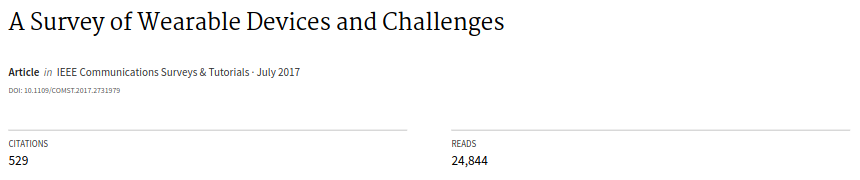
\includegraphics[width=1\linewidth]{imgs/ASurveyofWearableDevicesandChallenges}

\end{frame}


\subsection{Threats to Confidentiality}

\begin{frame}{Confidentiality}
	\begin{alertblock}{Definition}
	Threats to Confidentiality encompasses those where attackers get unauthorised  access to information using techniques such as eavesdropping  the wireless channel.	
	\end{alertblock}
	
	% 	Most existing wearable devices use Bluetooth Low Energy (BLE) as the major means of communication.
	
	
\end{frame}

\begin{frame}{Eavesdropping}
	\begin{itemize}
		\item Eavesdropping is the unauthorized real-time interception of a private communication which can expose user’s personal information to an attacker.
%Particularly, wearable devices using BLE communication protocol can suffer from eavesdropping.	
		\item The authors of the Open Effect Report from 2016 \cite{b7} investigated BLE privacy provision in number of fitness tracking devices such as Fitbit Charge HR, Jawbone UP 2, Garmin Vivosmart, 	Apple Watch, and Xiaomi Mi Band and came to the conclusion all tested devices, except Apple Watch, use the static device addresses that allowed attackers to \textbf{track user information such as location, time of fitness activities, and reversing user profile} by eavesdropping on these devices’ communications.
	\end{itemize}
\end{frame}

\begin{frame}{Traffic analysis}
	\begin{itemize}
		\item Traffic analysis attacks in the context of wearables involve monitoring communication patterns between devices.
		\item Privacy vulnerabilities have been identified in Bluetooth Low Energy (BLE) communication between fitness trackers and smartphones. 
		\item Adversaries can track users by analyzing BLE advertisements and static device addresses. 
		\item User activities can be inferred from the size and number of data packets in BLE traffic, even if the packets are encrypted. 
		\item Unique walking patterns can also be used to identify individuals within a small group, even with random 	addresses [1].
		\item It has been shown that the majority of fitness 		trackers use unchanged BLE addresses during advertising, 		making it feasible to track them. 
		\item The BLE traffic of the 		fitness trackers is found to be correlated with the intensity 		of the user’s activity, enabling an eavesdropper to determine 		the \textbf{user’s current activity} (walking, sitting, idle, or running) 		through analysis of the BLE traffic. 
	\end{itemize}
\end{frame}

\begin{frame}{Infomration Gathering Attacks.}
	\begin{itemize}
		\item Passive monitoring of wearable device transmissions enables adversaries to collect data exchanged between wearables and their hubs. 
		\item This information can be used for information gathering attacks, including breaking key exchanges in Bluetooth Low Energy (BLE) pairing and gathering information about user's other devices. 
		\item Researchers have demonstrated attacks that break BLE legacy pairing, infer keystrokes on smartphone touchpads using smartwatch motion sensors, decode keystrokes on keyboards using smartwatch sensors, and infer a user's personal PIN sequence using wearable devices.
		\item Adversaries can gain access to smartwatches by installing malicious applications to record sensor activities. 
		\item These attacks leverage sensor data captured by wearables and can be executed by sniffing BLE communications or installing malicious apps on wearables \cite{b1}.
	\end{itemize}
\end{frame}

\subsection{Integrity}


\begin{frame}{Threats to Integrity}
		\begin{alertblock}{Definiton}
			Threats to Integrity includes the cases  where attackers alter data or information without authorisation.  Threats to Availability are the situations where attackers act  to deny services to the entities who are authorised to use them.
		\end{alertblock}
	
		%Integrity is a crucial security requirement for wearable systems, particularly due to the sensitivity and privacy of the collected data. 	
		%Ensuring that data remains unaltered during transmission and reaches only authorized parties is paramount.	 
		%Various studies in the literature have evaluated the integrity of 		wearable device systems, identifying vulnerabilities in three attack categories: Modification Attacks, Replay Attacks, and Masquerade Attacks [1]. Additionally, this section comprises an overview of possible data breaches.
\end{frame}

¸TODO: Doch lieber nur eine Folie für alle attacken nehmen...

\begin{frame}{Make Titles Informative.}
\end{frame}

\begin{frame}{Make Titles Informative.}
\end{frame}



\subsection{Availability}

\begin{frame}

\begin{alertblock}{Definiton}
 Threats to Availability are the situations where attackers act  to deny services to the entities who are authorized to use them.
\end{alertblock}
\end{frame}


\section{Threats to security and privacy from accelerometer data}


\begin{frame}[fragile]{Threats to security and privacy from accelerometer data}
	
	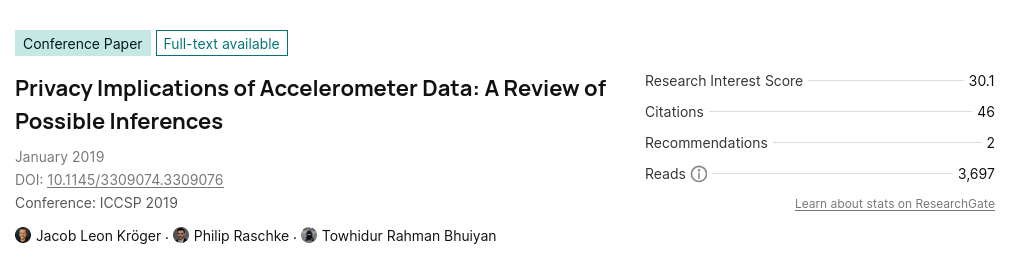
\includegraphics[width=1\linewidth]{imgs/Privacy Implications of Accelerometer Data A Review of Possible Inferences}
	
	% Particularly, privacy and security risks arise from the collection and utilization of accelerometer data on smartwatches and 	fitness trackers. The accelerometer, which measures motion 	and movement, can inadvertently disclose sensitive information about an individual’s activities and behavior. 
	% This data, if not properly protected, can be accessed by unauthorized parties and potentially lead to privacy or security breaches. Safeguarding the privacy of accelerometer data is crucial to ensure the confidentiality and security of users' personal information. 	The paper by Kröger et al. \cite{b5} is predestined for exemplifying that topic, since it highlights the potential privacy implications of accelerometers and security aspects such as inferring passwords, which are commonly found in mobile devices. While accelerometers are generally considered non-intrusive and do not require special permissions, research has shown that they can be used as a side channel to infer sensitive information about device holders. Accelerometer data alone can reveal details such as location, activities, health condition, body features, gender, age, personality traits, and emotional state. It can even be used for biometric identification and reconstructing text sequences, including passwords.
\end{frame}


\begin{frame}{Activity And Behavior Tracking}
% Accelerometers provide valuable data for a wide range of applications and can derive various physical activity variables and behavior-related information.
\begin{itemize}
	\item Accelerometers are used in step counters to estimate \textbf{energy expenditure} and \textbf{distance walked}, and in medical studies to assess \textbf{sedentary time and physical activity}.
	\item They enable real-time \textbf{body posture} and \textbf{activity
	classification}, including basic activities like running, walking,
	and sitting, as well as more complex activities like writing,
	typing, and painting. 
	\item They can also monitor \textbf{sleep patterns
	and behaviors}. 
	\item They can detect \textbf{hand 	gestures, eating and drinking moments, smoking, and even
	distinguish levels of intoxication}. 
	\item They have been used to detect \textbf{carried loads and estimate carried weight}, \textbf{measure driving behavior}, \textbf{analyze speech activity} and \textbf{social interactions}, and
	\textbf{reconstruct speech from recorded vibrations}. 
	%\item It has been observed that researchers were able to detect aggressive or 	unsafe driving styles and drunk driving patterns. 
 	% The potential applications of accelerometers are vast and extend to various	domains such as healthcare, fitness tracking, and behavior 	analysis [5].
\end{itemize}
\end{frame}


\begin{frame}{Location Tracking}
\begin{itemize}
	\item Studies have demonstrated that accelerometers in mobile
	devices can be utilized for \textbf{user localization and reconstruction
	of travel trajectories}, even in the absence of GPS or other localization systems.
	\item Researchers have achieved \textbf{geographically tracking individuals driving a car} solely based on accelerometer readings from their smartphones.
%  By analyzing three-axis acceleration measurements and mapping them to existing 	routes on a map, they obtained trajectory information with accuracy comparable to handheld GPS devices. 
	\item Another study focused on using smartphone accelerometers to determine the \textbf{location of the user within a metropolitan train system}. 
	%By comparing acceleration patterns with labeled training data, specific station intervals were recognized, and the accuracy	of the approach reached up to 89% for rides longer than 3 stations and 92% for rides longer than 5 stations. These 	findings highlight the potential privacy risks associated with 	accelerometer data and the ability to infer sensitive information about individuals’ whereabouts and travel patterns [5].
\end{itemize}
\end{frame}


\begin{frame}{User Identification}
\begin{itemize}
	\item Ability to differentiate between and uniquely identify users
	\textbf{based on their body movement patterns}. 
	\item Biometric features such as \textbf{gait, hand gestures, and head movements}  have been used for user identification with high
	accuracy. % For example, one study achieved 100% accuracy in recognizing individuals from a test group using accelerometer readings from smartphones. 
	\item Capability distinguish between different speakers accurately by sound vibrations, including human speech, with enough quality to .
	\item The trajectory of a mobile device can reveal a \textbf{user’s work and home addresses}. 
	\item When combined with other auxiliary datasets, such as white pages
	or employment directories, it can potentially expose a user’s
	real identity.
	%\item Device fingerprinting techniques can further differentiate users based on unique characteristics of their personal devices. 
	\item Calibration errors in accelerometers %, caused by manufacturing imperfections,
	have been found sufficient to create a device ”fingerprint” that can track users across website visits, even when other tracking technologies like cookies are
	blocked.
\end{itemize}
\end{frame}


\begin{frame}{Keystroke Logging}
  \begin{itemize}
  	\item The input that users type into their devices, whether through touchscreens or keyboards, often contains highly sensitive information such as text messages, personal notes, login credentials, and transaction details. 
  	% Researchers have shown that motion sensor data can be used to reconstruct user inputs from handheld and wrist-worn devices.
  	%By analyzing the hand movements associated with swipes, taps, and keystrokes, researchers have successfully inferred inputs from motion sensor data. 
  	\item Researchers have demonstrated to infer tap- and gesture-based inputs, including \textbf{PINs and graphical password patterns}. 
  	\item Entire sequences of text entered through a phone’s touchscreen have been obtained using accelerometer data. 
  	%\item The fact that even multi-sensor attacks predominantly use acceleration information for tap detection highlights the importance of focusing on defense mechanisms against these types of side-channel attacks, particularly in relation to accelerometers
  	\pause
  	\item \alert{Later we will talk about a paper that particularly facing the topic of inferring typed words.}
  \end{itemize}
\end{frame}


\begin{frame}{Inference of Health Parameters and Body Features}
\begin{itemize}
	%Body-worn accelerometers provide valuable insights into a person’s physical characteristics and health status. 
	\item By analyzing accelerometer data from smartphones, researchers have
	been able to approximate  \textbf{users’ body weight and height}.
	% \item There is a strong correlation between accelerometer-determined	physical activity and obesity, making physical activity a recognized \textbf{indicator of health}. 
	\item The amount of physical activity can reveal information about \textbf{latent chronic diseases, mobility, cognitive function, and even the risk of mortality}.
	\item Accelerometer data allows for the derivation of various
	activity-related variables such as \textbf{energy expenditure, activity type, and temporal activity patterns}.
	% These variables are 	increasingly used in health studies to remotely assess participants’ physical activity levels. 
	\item Sleep duration is anotherimportant factor in population health, and accelerometers in	wearable devices have been utilized to evaluate \textbf{sleep patterns, fragmentation, and efficiency}. 
	\item Specialized accelerometers have been employed to measure additional health parameters, including \textbf{voice health, postural stability, and physiological sound}. 
	% The versatility of accelerometers makes them valuable in monitoring various 	aspects of an individual’s well-being and can aid in healthcare	research and personalized healthcare management [5].
\end{itemize}.
\end{frame}


\begin{frame}{Inference of Demographics}
 \begin{itemize}
	\item Data from body-worn accelerometers can be used to estimate demographic variables such as \textbf{age and gender}.  
	%Gait features, including step length, velocity, and step timing variability,	vary between younger and older subjects. 	
	%Hip movements, gait features, and 	physical activity patterns derived from accelerometers can be 	used to estimate the sex of individuals.
	\item Differences in \textbf{walking smoothness} between adults and children
	can be detected through accelerometer readings. 
%	\item 	Using smartphone accelerometer data, researchers have achieved a 92.5\% success	rate in predicting the \textbf{age interval} of test subjects based on their	smartphone holding and touching behaviors.
	\item  Notably, accelerometer-based gender recognition can work independently of a person’s weight and height. 
	\item Additionally, acoustic vibrations captured
	through a smartphone accelerometer can be used to classify
	speakers as male or female with high accuracy.
 \end{itemize}
\end{frame}


\begin{frame}{Mood and Emotion Recognition}
	\begin{itemize}
		\item Physical activity, as measured by body-worn accelerometers, has been linked to human emotions and depressive moods. 
		\item Researchers have used accelerometer data from smart
		wristbands to recognize emotional states, such as \textbf{happiness,
		neutrality, and anger}, with fair accuracy.
		\item  Accelerometers in smartphones have been employed to detect \textbf{stress levels and arousal in users}. 
		\item Additionally, there is a positive association between accelerometer-derived s\textbf{peech activity and mood changes}.
	\end{itemize}
\end{frame}



\begin{frame}{Inference of Personality Traits}
	\begin{itemize}
 		\item Methods have been developed to infer \textbf{preferences and
 		personality traits} based on body gestures and motion patterns
 		captured by accelerometers. 
 		\item Wearable accelerometers were
 		used to estimate the \textbf{motivations, interests, and group affiliations} of study participants during social interactions, relying
 		on their movements, body postures, and gesturing patterns.
 		
 		\item % Furthermore, a person’s level of physical activity, which can be measured using body-worn accelerometers, has been found to correlate with specific personality traits.
 		Studies have shown that \textbf{conscientiousness, neuroticism, openness, and
 		extraversion} are associated with different levels of physical
 		activity. %For example, it has been found that agreeableness, 		conscientiousness, and extraversion were positively correlated with higher step counts and physical activity variables, whileneuroticism showed a negative association.
 		\item Moreover, it has been discovered that neuroticism and the functioning of the
 		behavioral inhibition system were related to physical activity
 		measures derived from accelerometer data in female college
 		students.
	\end{itemize}
\end{frame}


\section{Inferring Typed Words}

\begin{frame}{Inferring Typed Words}
	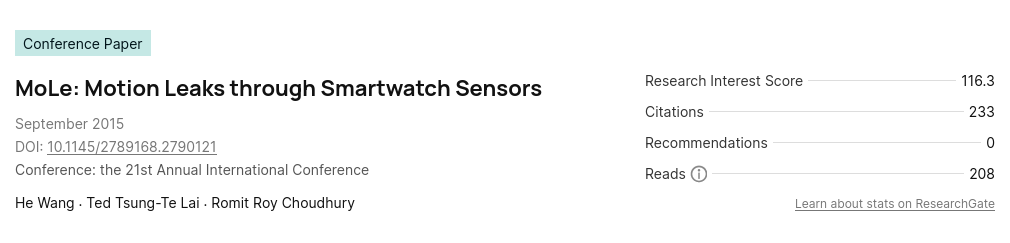
\includegraphics[width=1\linewidth]{imgs/MoLePaper}
\end{frame}


\begin{frame}
 \begin{itemize}
 	\item The paper highlights the significant ramifications
 	of such data leakage, as smartwatches can be camouflaged
 	as activity trackers, thereby compromising the privacy of a
 	\textbf{user’s emails, search queries, and other documents typed} on
 	the keyboard. 
 	
 	%Given the importance of addressing privacy and  	security risks associated with accelerometer data, this paper  	has been selected for further investigation and analysis.
 	\item %Unlike keystroke loggers that need to find loopholes in the 	operating system, 
 	The activity tracker malware can obtain the	user’s permission and easily launch a side channel attack. 	
 \end{itemize}
\end{frame}

\begin{frame}{Assumptions and Constraints}
	\begin{itemize}
		\item Smartwatch is worn on the left hand.
		\item The absence of data from the right hand is a unique constraint, and so it needs to infer which finger	executed the key-press.
		\item For a given position of the wrist watch, it is not obvious which one of the 3 or 4 different keys could have been pressed, which could be further interspersed by unknown number of keys pressed by the right hand. 
		\item Users write different with dexterity, e.g. some use their little
		finger far less efficiently while others use specific fingers when
		it comes to digits or corner keys.
	\end{itemize}
\end{frame}

\begin{frame}{Data Collection}
	Inhalt...
	
		Two authors put on Samsung Gear Live
	smart watches and typed 500 words each wearing the smart
	watch on their left wrist. The accelerometer and gyroscope
	data is used as training data, and processed through a sequence
	of steps, including key-press detection, hand-motion tracking,
	character point cloud computation, and Bayesian modeling and
	inference. The test data was collect by 8 different volunteers
	who were asked to type 300 different English words from a
	dictionary. The smart-watch sensor data from the volunteers
	was used to create a short-lists K words, ranked in the
	decreasing order of probability (i.e., the first ranked word is
	considered the most probable guess) [3].
	
\end{frame}


\section*{Summary}

\begin{frame}{Take Home Messages}

  % Keep the summary *very short*.
  \begin{itemize}
  \item
    The \alert{first main message} of your talk in one or two lines.
  \item
    The \alert{second main message} of your talk in one or two lines.
  \item
    Perhaps a \alert{third message}, but not more than that.
  \end{itemize}
  
  % The following outlook is optional.
  \vskip0pt plus.5fill
  \begin{itemize}
  \item
    Outlook
    \begin{itemize}
    \item
      Something you haven't solved.
    \item
      Something else you haven't solved.
    \end{itemize}
  \end{itemize}
\end{frame}



% All of the following is optional and typically not needed. 
\appendix
\section<presentation>*{\appendixname}
\subsection<presentation>*{For Further Reading}

\begin{frame}[allowframebreaks]
  \frametitle<presentation>{For Further Reading}
    
  \begin{thebibliography}{10}
    
  \beamertemplatebookbibitems
  % Start with overview books.

  \bibitem{Author1990}
    A.~Author.
    \newblock {\em Handbook of Everything}.
    \newblock Some Press, 1990.
 
    
  \beamertemplatearticlebibitems
  % Followed by interesting articles. Keep the list short. 

  \bibitem{Someone2000}
    S.~Someone.
    \newblock On this and that.
    \newblock {\em Journal of This and That}, 2(1):50--100,
    2000.
  \end{thebibliography}
\end{frame}

\end{document}
